\chapter{Trigger categories}
\label{appx:trigger-cat}

\Cref{fig:trigger-cat} and the text in this appendix are paraphrased from
\cite{LHCb-PUB-2014-039}.
It is included for completeness of this document.

\begin{figure}[htb]
    \centering
    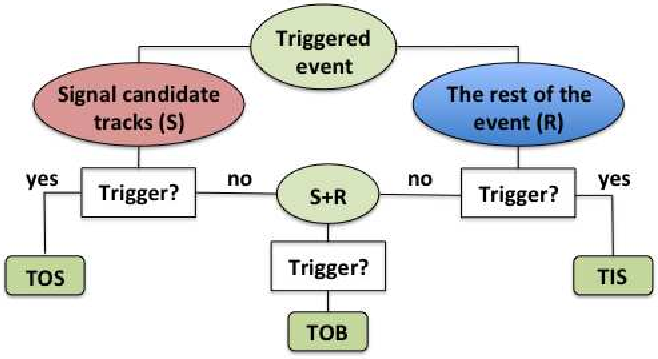
\includegraphics[width=0.5\textwidth]{./figs-trigger-categories/trigger_categories.pdf}
    \caption{Schematic of the trigger categories.}
    \label{fig:trigger-cat}
\end{figure}

\begin{itemize}
    \item Trigger On Signal (TOS): The signal track (and its decay chain) alone
        is sufficient to fire the trigger.
    \item Trigger Independent of Signal (TIS): The rest of event alone is
        sufficient to fire the trigger.
    \item TISTOS: Both signal and the rest of event alone are sufficient to
        generate a positive trigger decision.
    \item Trigger On Both (TOB): Neither signal nor the rest of event alone is
        sufficient to generate a positive trigger decision, only the combination
        is.
        Note that all event must have a positive trigger decision for it to be
        saved.
\end{itemize}
